\documentclass[tikz,border=5mm,12pt]{standalone}
\usepackage[fontsize=16pt]{fontsize}

\newcommand\sep{14mm}

\newcommand\setcoordinates{
  \path (0,0) coordinate (P1)
    -- ++(360-22.5:\sep) coordinate (P2)
    -- ++(360-22.5-45:\sep) coordinate (P3)
    -- ++(360-22.5-90:\sep) coordinate (P4)
    -- ++(360-22.5-135:\sep) coordinate (P5)
    -- ++(360-22.5-180:\sep) coordinate (P6)
    -- ++(360-22.5-180-45:\sep) coordinate (P7)
    -- ++(360-22.5-180-90:\sep) coordinate (P8);
}
\newcommand\drawnodes{
  \node[person] at (P1) {1};
  \node[person] at (P2) {2};
  \node[person] at (P3) {3};
  \node[person] at (P4) {4};
  \node[person] at (P5) {5};
  \node[person] at (P6) {6};
  \node[person] at (P7) {7};
  \node[person] at (P8) {8};
}

\begin{document}
  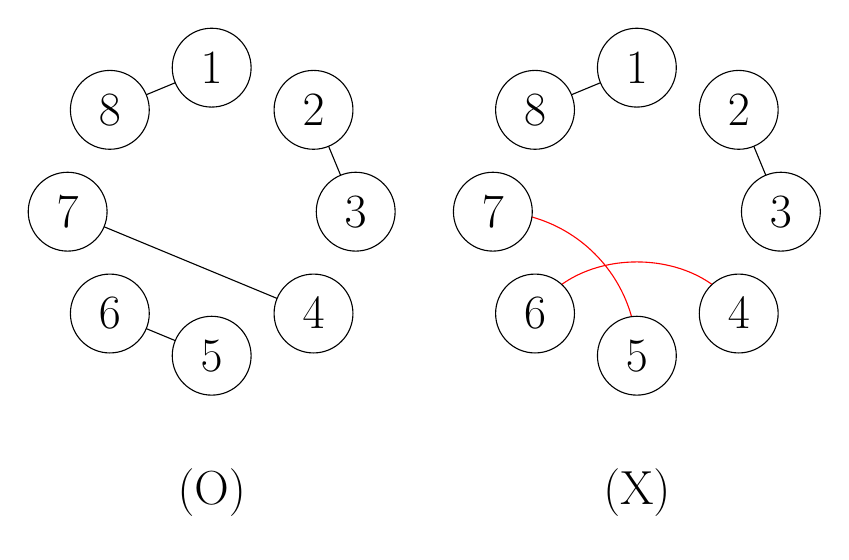
\begin{tikzpicture}[
    person/.style={draw,circle,fill=white}
  ]
    \begin{scope}
      \setcoordinates;

      \draw (P1) -- (P8);
      \draw (P2) -- (P3);
      \draw (P4) -- (P7);
      \draw (P5) -- (P6);

      \drawnodes

      \node at (0,-54mm) {(O)};
    \end{scope}

    \begin{scope}[xshift=54mm]
      \setcoordinates;

      \draw (P1) -- (P8);
      \draw (P2) -- (P3);
      \draw[red] (P4) to[out=120,in=60] (P6);
      \draw[red] (P5) to[out=90,in=0] (P7);

      \drawnodes

      \node at (0,-54mm) {(X)};
    \end{scope}
  \end{tikzpicture}
\end{document}
